\documentclass[12pt]{article}
\usepackage{amssymb}
\usepackage[UTF8]{ctex}
\usepackage{geometry}
\usepackage{units}
\usepackage{pifont}
\geometry{
	a4paper,
	total={150mm,237mm},
	left=30mm,
	top=27mm,
	}
\usepackage{amsmath}
\usepackage{enumerate}
\usepackage{lipsum}
\usepackage{graphicx}
\usepackage{hyperref}
\usepackage{indentfirst}
\usepackage[graphicx]{realboxes}
\usepackage{booktabs}
\usepackage{cases}
\usepackage{subfig}  
\usepackage{float}
\usepackage{xcolor}
\setlength{\parindent}{2em}
\title{Lab3}
\author{姓名:陈锐林,学号:21307130148}
\date{\today}

\begin{document}
\maketitle
\begin{Large}
	\noindent 实验1:加速系统调用速度\par
\end{Large}
\noindent
\hspace*{2em}0.这里在ppt里已经给出了完整的实现过程,所以就跟着ppt,记录每个步骤的做法和代码。\par
1.添加指针保存页表地址。根据hint,我们可以通过struct usycall实现映射;并利用已经实现的函数。查阅memlayout.h,usycall已经定义好了,包含一个成员pid。
所以在proc的定义中添上如下代码即可:
\begin{figure}[h]
	\centering
	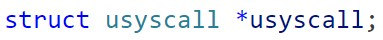
\includegraphics[height=0.8cm,width=6cm]{lab3-1.jpg}
\end{figure}\\
\hspace*{2em}2.这步要求为上面定义的usycall分配空间,并初始化pid。翻看allocproc()的其余部分可以很快学习到写法,先用kalloc尝试分配,如果出错,解锁并return。初始化pid,应该是将p->pid给p->usycall,这里用memmove应该就可以了。代码如下:
\begin{figure}[h]
	\centering
	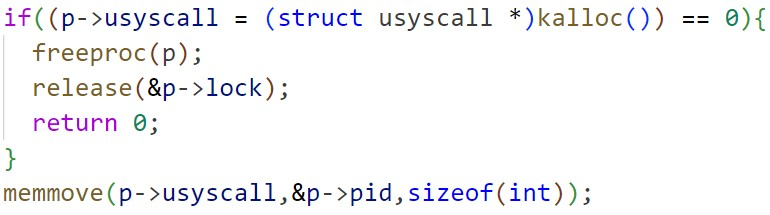
\includegraphics[height=4cm,width=10cm]{lab3-2.jpg}
\end{figure}\\
\hspace*{2em}3.这步要求将该PTE写入pagetable,设置为用户可读。观察到,proc\_pagetable这个函数的书写逻辑,和allocproc是有点像的;都是if里尝试mappages一个东西,如果失败;就要free。
该函数中先mappages TRAMPOLINE,失败则释放(uvmfree)页表;再mappages TRAPFRAME,如果失败要解开映射(uvmunmap),再释放(uvmfree)页表。所以我们可以把对于PTE的写入放在最后,如果失败,先uvmunmap TRAMPOLINE 和 TRAPFRAME,再uvmfree页表。
至于用户权限,riscv.h有写,该用PTE\_R | PTE\_U。最后代码如下:
\newpage
\begin{figure}[h]
	\centering
	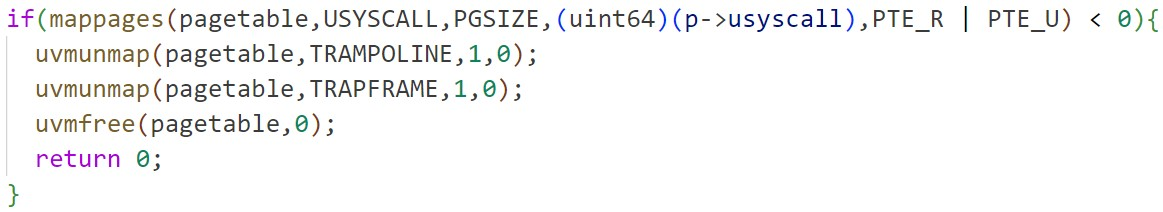
\includegraphics[height=4.5cm,width=15cm]{lab3-3.jpg}
\end{figure}

4.这步要让freeproc能释放共享页,并插入空闲页链表。这里在函数开始就kfree,并且将该usycall指向的pid置0即可。最后代码如下:
\begin{figure}[h]
	\centering
	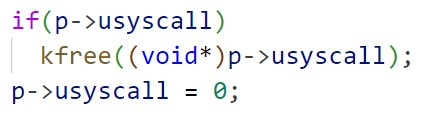
\includegraphics[height=2.5cm,width=6.25cm]{lab3-4.jpg}
\end{figure}\\
\hspace*{2em}5.这步解除映射关系,观察proc\_freepagetable内的其他部分。同样对usycall进行uvmunmap即可。最后代码如下:
\begin{figure}[h]
	\centering
	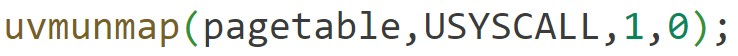
\includegraphics[height=1cm,width=6.5cm]{lab3-5.jpg}
\end{figure}\\
\hspace*{2em}6.测试结果,运行pgtbltest可以看到通过测试。如下:\\
\begin{figure}[H]
	\centering
	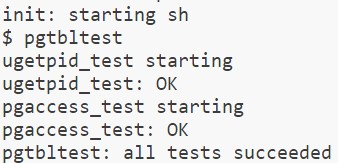
\includegraphics[height=5cm,width=9cm]{lab3-6.jpg}
\end{figure}

\begin{Large}
	\noindent 实验2:打印页表\par
\end{Large}
1.在def.h中如下定义即可,其中第二个int表示递归层数,这是由后面的代码决定的;与ppt不同,但是无伤大雅,可以不用再定义新函数。
\newpage
\begin{figure}[h]
	\centering
	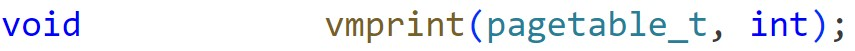
\includegraphics[height=1cm,width=7cm]{lab3-7.jpg}
\end{figure}
2.vmprint函数是这个实验的关键,根据hint,参考freewalk函数;我们可以知道是要考虑递归的树状结构。递归的思路就是一级一级调用vmprint();而因为是多级页表,所以要做出区分,到底是不是叶节点。如果是叶结点就结束递归。
怎么区分成了一个问题,但是看懂freewalk函数后就发现,情况是一样的。所以对freewalk函数进行一个拙劣的模仿就好了,级数level用来控制..生成的数量。其他的就是PTE2PA生成孩子,按照样例打印。代码如下:
\begin{figure}[h]
	\centering
	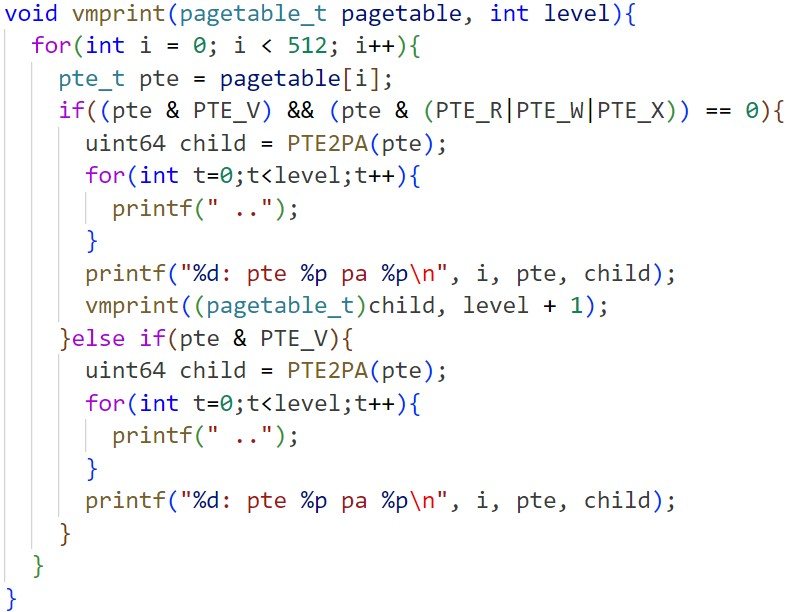
\includegraphics[height=8cm,width=11.25cm]{lab3-8.jpg}
\end{figure}\par
3.这里就是添加,没什么不一样的。但是我把题目要求的page table这一行挪到这了(当然在vmprint中判断level来解决也可以qwq)。\\
\hspace*{2em}4.测试结果如下:其中左侧make grade包含三个实验测试
\begin{figure*}[!h]
    \centering
    \subfloat[]{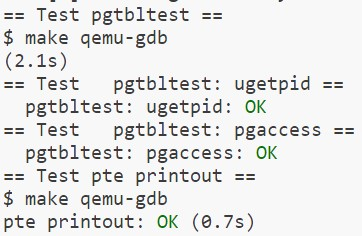
\includegraphics[width=4cm,height=5cm]{lab3-9.jpg} \label{X}}
    \hfill
    \subfloat[]{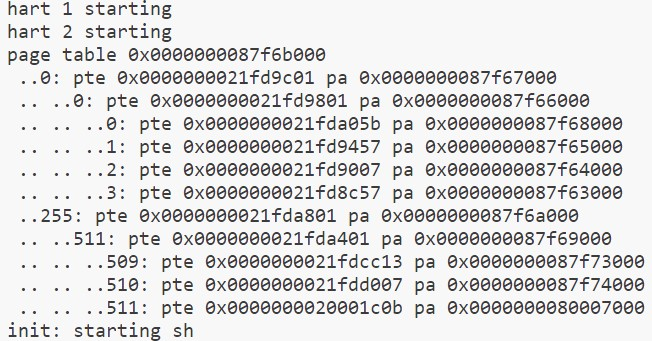
\includegraphics[width=7cm,height=5cm]{lab3-11.jpg} \label{Y}}
\end{figure*}
\newpage
\begin{Large}
	\noindent 实验3:检测哪些页被访问\\
\end{Large}
1.这步实现sys\_pgaccess(),具体分为以下部分:\par
(1)根据题意,这个函数接受三个参数,用户页起始虚拟地址(定义为vp),被检查页数(Numpages),用户空间地址(ua)。
我们可以用argaddr和argint导入。\par
(2)Numpages可设上限,取为64,超过就取64。\par
(3)定义变量mask表示掩码;获取方式如下:对于范围在当前页开始的Numpages内的所有页,通过walk函数寻找页表项;只要正确找到,就考察是否被访问(PTE\_A),如果访问过了要及时清除(对PTE\_A取反再与)。\par
(4)最后用copyout把mask送到ua。\par
(5)代码如下:\\
\begin{figure}[h]
	\centering
	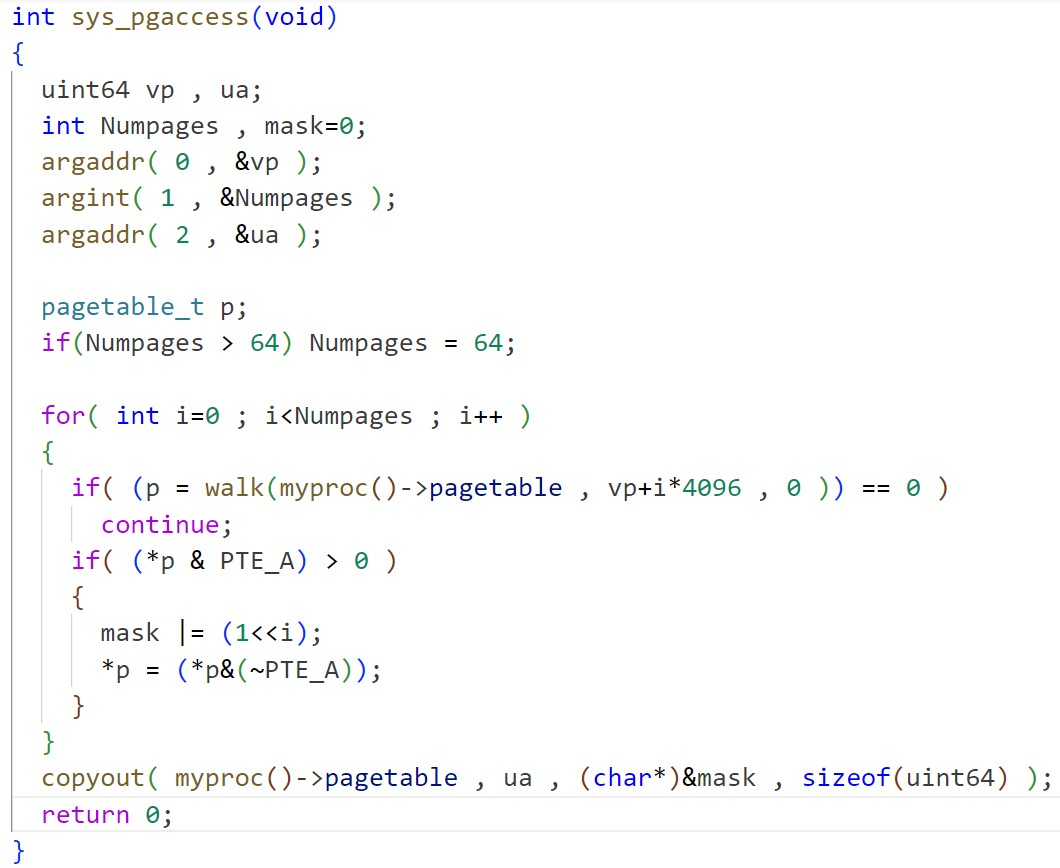
\includegraphics[height=8cm,width=12cm]{lab3-12.jpg}
\end{figure}\\
2.设置PTE\_A,这里要根据RISCV架构,经查询(如下)应该是 1 << 6。\\
\begin{figure}[h]
	\centering
	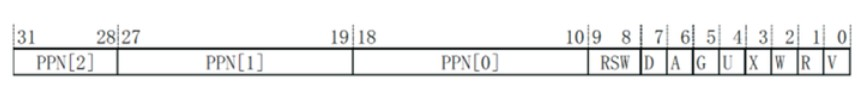
\includegraphics[height=1cm,width=8cm]{lab3-10.jpg}
\end{figure}\\
3.运行效果,在实验1已展示:
\begin{figure}[H]
	\centering
	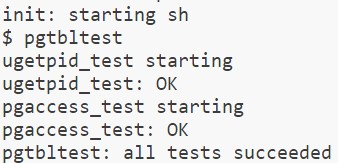
\includegraphics[height=3cm,width=4cm]{lab3-6.jpg}
\end{figure}
\end{document}